\chapter{Architektur}
\label{chap:architektur}

In diesem Kapitel wird die Architektur des Projekts beschrieben. 

\section{Überblick}
Die Gesamtarchitektur gliedert sich in mehrere Teilsysteme, die zusammenarbeiten, um ein stabiles Mehrspieler-Erlebnis zu gewährleisten. 
Das Spiel selbst läuft in Godot-Instanzen (Game-Server), die durch zentrale Backend-Komponenten verwaltet werden. 
Die Kommunikation erfolgt über klar definierte Schnittstellen zwischen Frontend, Loadbalancer, Masterserver, Datenbanken und Game-Servern. 
Ein schematischer Überblick ist in Abbildung~\ref{fig:architektur} dargestellt.

\begin{figure}[h!]
  \centering
  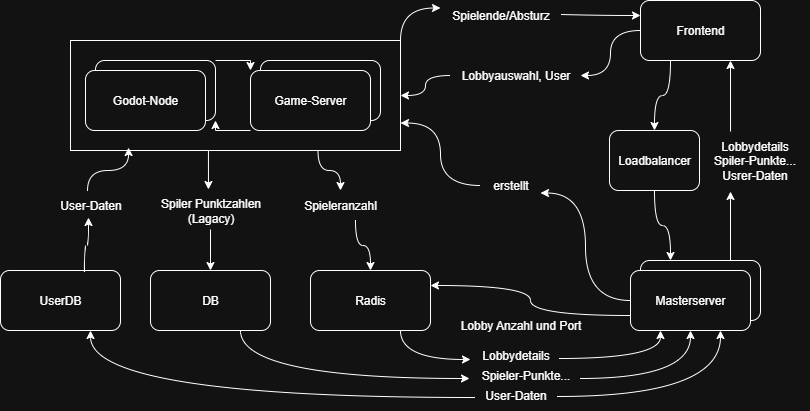
\includegraphics[width=0.95\linewidth]{../images/content.png}
  \caption{Architekturübersicht des Projekts}
  \label{fig:architektur}
\end{figure}


Bei der Planung der Architektur wurde stets darauf geachtet für den Benutzer die bestmögliche Erfahrung zu schaffen.
Hierfür wurde sich für WebSockets entschieden, um es dem Spieler zu ermöglichebn einfach im Browser zu spielen, ohne zusätzliche Software installieren zu müssen.
WebSockets bieten eine durchgehende Verbindung, bei der Client und Server jederzeit Daten senden können, was bei Echtzeit-Anwendungen wie Spielen die Verzögerung deutlich reduziert.
Vgl. hierzu auch:
(Alex Booker: *WebSockets vs HTTP: Which to choose for your project in 2024*, Ably, 13 min read \url{https://ably.com/topic/websockets-vs-http} (letzter Zugriff: 17.09.2025))


\section{Frontend}
Das Frontend stellt die Schnittstelle zum Spieler dar. 
Hier können Lobbys ausgewählt, Benutzer eingeloggt und Spieldetails angezeigt werden. 
Nach Spielende oder im Falle eines Absturzes liefert das Frontend entsprechendes Feedback an den Benutzer.
Dieses wurde in Angular umgesetzt und kommuniziert über HTTP und WebSockets mit dem Backend.
Angular wurde ausgewählt, da es eine moderne, komponentenbasierte Struktur bietet und die Entwicklung von Single-Page-Applications (SPAs) erleichtert. 
Außerdem war Angular bereits aus vorherigen Projekten bekannt, was die Einarbeitungszeit verkürzte.
\noindent
Vgl. hierzu auch:  
Sparkout Tech Solutions: \textit{Angular: Modern Web Application Development}, Medium, 28. Oktober 2023.  
URL: \url{https://sparkouttechsolutions.medium.com/angular-modern-web-application-development-ac2b3acdc878} (letzter Zugriff: 17.09.2025)


\section{Loadbalancer}
Der Loadbalancer verteilt eingehende Anfragen auf die verfügbaren Game-Server. 
Er sorgt dafür, dass neue Lobbys erstellt werden können und die Last gleichmäßig über mehrere Server verteilt wird. 
Dadurch wird die Skalierbarkeit des Systems gewährleistet.
Dieser wurde mit Nginx realisiert, da es eine bewährte Lösung für Lastverteilung darstellt. 
Es können beim Start der Container beliebig viele Masterserver-Instanzen angegeben werden. 
Dies geschieht unter dem Docker-Compose-Flag --scale masterserver=Anzahl. 

\section{Masterserver}
Der Masterserver (in Express) übernimmt die zentrale Verwaltung aller Lobbys und handhabt Informationen zu:
\begin{itemize}
  \item Anzahl und Ports der Lobbys,
  \item Spielern und deren Punkteständen,
  \item Metadaten wie Spielstatus und Benutzerinformationen.
\end{itemize}
Diese Daten werden sowohl an das Frontend als auch an die Game-Server weitergegeben.

\section{Game-Server und Godot}
Die eigentliche Spiellogik läuft in den Godot nodes, welche dann als HTML5 exportiert werden.
Das exportierte Spiel wird dann über die Game-Server dynamisch für den Client bereitgestellt. 
Jeder Game-Server repräsentiert eine Lobby und übernimmt die Synchronisation der Spielzustände zwischen den Spielern. 
Die Game-Server kommunizieren kontinuierlich über einen Redis-Cache mit dem Masterserver, um Daten wie Spieleranzahlen und Statusmeldungen zu übermitteln.
Die Punktestände sowie Userdaten werden in einer seperaten relationalen Datenbank gespeichert.

\section{Datenbanken}
Zur Verwaltung werden zwei Datenbanken eingesetzt:
\begin{itemize}
  \item \textbf{UserDB}: Speicherung von Benutzerinformationen wie Username und gehashtem Passwort in einer PostgreSQL-Datenbank. 
  \item \textbf{LeaderboardDB}: Speicherung von Spielerpunktzahlen und gespielten Spielen in einer PostgreSQL-Datenbank.
  \item \textbf{Redis}: Speicherung von Lobbydetails und temporären Statusdaten für schnelle Zugriffe und Synchronisation zwischen Masterserver und Game-Servern.
\end{itemize}

\section{Zusammenspiel}
Das Zusammenspiel der Komponenten erfolgt in folgenden Schritten:
\begin{enumerate}
  \item Ein Spieler wählt im Frontend eine Lobby aus oder erstellt eine neue.
  \item Der Loadbalancer leitet die Anfrage an den Masterserver weiter.
  \item Der Masterserver erstellt eine Lobby auf einem Game-Server und verwaltet alle relevanten Metadaten.
  \item Während des Spiels werden kontinuierlich Statusdaten (z.\,B. Punktestände, Spieleranzahlen) zwischen Game-Server, Redis und Masterserver ausgetauscht.
  \item Nach Spielende oder einem Absturz werden die Daten an das Frontend zurückgemeldet und gespeichert.
\end{enumerate}